%!TEX root = ../main.tex

%\documentclass[twoside,twocolumn,a4j,dvipdfmx]{jarticle}
%\usepackage{amsmath,amssymb}
%\usepackage[dvipdfmx]{graphicx}
%\newcommand{\im}{\mathrm{i}}
%\newcommand{\bx}{\mathrm x}
%\begin{document}

常微分方程式の一つであるvan der Pol方程式の周期解の数値計算をまず行い、得た近似解をもとに解の精度保証を行う。

\subsection{van der Pol 方程式}
van der Pol方程式とは、以下のような方程式である。
$$
\frac{d^2 x}{dt^2} - \mu (1-x^2)\frac{dx}{dt} + x = 0.
$$
ここで、$x(t)$ が未知関数で、$\mu>0$ は非線形の減衰の強さを表すパラメータである。van der Pol 方程式を次の連立常微分方程式系にして\texttt{DifferentialEquations.jl}のというJulia言語のパッケージ\cite{DEjl}に実装されているODEソルバーで数値計算する。
$$
\begin{cases}
\dot{x} = y\\
\dot{y} = \mu (1-x^2)y - x.
\end{cases}
$$
初期値は $x(0)=0$, $y(0)=2$とし, $\mu=1$ とする。

%%
\begin{comment}
\begin{verbatim}
using DifferentialEquations

function vanderpol(du, u , μ ,t)
    x,y = u
    du[1] = y
    du[2] = μ*(1- x ^2)*y - x
end

u0 = [0.0; 2.0]
tspan = (0.0, 300)
μ = 1.0
prob = ODEProblem(vanderpol, u0, tspan, μ)
sol = solve(prob,Tsit5(),
           reltol=1e-8,abstol=1e-8)
\end{verbatim}
\end{comment}

\begin{comment}
\subsection{Newton法の初期値の設定}

まず、フーリエ級数の係数を求めるために、van der Pol方程式の周期解の周期を大まかに求める。

\begin{verbatim}
a = 30
app_period = 6.55
timestep = 0.1

f_tmp = sol(a+app_period/2:timestep:a
               +3*app_period/2)
find_period = abs.(f_tmp .- sol(a))
(~,ind) = findmin(find_period[1,:])
b = a+app_period/2 + timestep*(ind-1)
\end{verbatim}
\end{comment}
%%

\subsection{Newton法を用いた周期解の求め方}

van der Pol方程式は、$\dot{x} = \frac{dx}{dt}$とおくと、以下のように表すことができる。
$$
\ddot{x} - \mu(1-x^2)\dot{x} + x = 0.
$$
後の計算のために、式を少し整理すると、
$$
\ddot{x} - \mu\dot{x} + \frac{\mu}{3} \dot{(x^3)} + x = 0
$$
と書ける。また、周期解$x(t)$を周期$L$の周期関数とし、$\omega = \frac{2\pi}{L}$とおくと、$x(t)$とその微分や$2$乗はフーリエ級数を使って、
\begin{align*}
x(t) &= \sum_{k \in \mathbb{Z}} a_k e^{\im k\omega t}\\
\frac{dx(t)}{dt} &= \sum_{k \in \mathbb{Z}}(\im k \omega) a_k e^{\im k \omega t} \\
\frac{d^2 x(t)}{dt^2} &= \sum_{k \in \mathbb{Z}} (-  k^2 \omega^2 )a_k e^{\im k\omega t} \\
x(t)^3 &= \sum_{k \in \mathbb{Z}} (a * a * a)_k e^{\im k \omega t}
\end{align*}
と書くことができる。ここで
\begin{equation*}
(a^3)_k := \sum_{\substack{k_1+k_2+k_3 = k\\k_i\in\mathbb{Z}}} a_{k_1}a_{k_2}
a_{k_3},\quad k\in\mathbb{Z}
\end{equation*}
は3次の離散たたみこみである。

以上の式を用いて、フーリエ係数に関する式を立てる。$a = (a_k)_{k \in \mathbb{Z}}$に対して、van der Pol方程式に求めたフーリエ級数を代入すると、
$$
f_k(a) := -k^2\omega^2 a_k - \mu\im k \omega a_k + \frac{\mu }{3}(\im k \omega)(a*a*a)_k + a_k
$$
となる点列 $\left(f_k(a)\right)_{k\in\mathbb{Z}}$が得られる。そして、点列 $a$ がvan der Pol方程式の解のフーリエ係数になっているならば、各 $k\in\mathbb{Z}$ について
$$
f_k(a) = 0
$$
となる。このときの未知数は周波数 $\omega$ と点列 $a$ であり、これらを並べて $\bx = (\omega,a)$ と書くことにする。未知数 $\bx$ に対して、$f_k(a) = 0$ という方程式だけでは不定な方程式になるため、解の形を一つに定める事ができない。そこで、位相条件
\begin{equation*}
    \eta (a) := \sum_{|k|<N} a_k - \eta_0=0, \quad \eta_0 \in \mathbb{R} 
\end{equation*}
を加える。この条件は $x(t)$ の初期値 $x(0) = \eta_0$ を表している。最終的に van der Pol 方程式の周期解の求解は次の代数方程式を解くことに帰着される。
$$
    F(\bx) := 
    \begin{bmatrix}
    \eta (a) \\
    (f_k(a)_{k\in\mathbb{Z}}
    \end{bmatrix}
    =0.
$$

以下、この零点探索問題 $F(\bx)=0$ について Newton 法で解を得ることを考える。まず $N$ をフーリエ係数の打ち切り番号(最大波数:$N-1$)とし、周期解の近似を次のように構成する。
$$
 \bar{x}(t) = \sum_{|k|<N} \bar{a}_k e^{\im k \bar\omega t}.
$$

このとき、フーリエ係数と(近似)周期を並べた
$$
    \bar{\bx} = (\bar\omega, \bar{a}_{-N+1},\dots,\bar{a}_{N-1})\in \mathbb{C}^{2N}
$$
を近似解とよぶ。近似解 $\bar \bx$ の未知数は $2N$ 個。そして $f_k(a)=0$ を $|k|<N$ の範囲で打ち切る方程式
$$
    F^{(N)}(\bx^{(N)}) = 
    \begin{bmatrix}
    \eta (a^{(N)}) \\
    (f_k(a^{(N)}))_{k < |N|}
    \end{bmatrix}
    =0
$$
を考える。ここで $a^{(N)} = (a_k)_{|k|<N}$, $\bx^{(N)} = (\omega,a^{(N)})$ をそれぞれ表し、$F^{(N)}:\mathbb{C}^{2N}\to \mathbb{C}^{2N}$ である。したがって $F^{(N)}(\bx^{(N)}) = 0$ という有限次元の非線形方程式を解くことで、近似解 $\bar \bx$ が得られる。

\subsection{Newton法による周期解の数値計算}

Newton法の式は、ある適当な初期値 $\bx_0$ を最初に定め、以下の反復計算によって計算できる。
$$
    \bx_{n+1} = \bx_n - DF^{(N)}(\bx_n)^{-1} F^{(N)}(\bx_n),\quad n=0,1,\dots
$$

このことから、$DF^{(N)}(\bx_n)^{-1}$ と $F^{(N)}(\bx_n)$ を計算することができれば、近似解を得ることができる。そして、$F^{(N)}(\bx^{(N)})$のヤコビ行列は、
\begin{align*}
    DF^{(N)}(\bx^{(N)}) = 
    \left[\begin{array}{c|ccc}
    0 & 1 & \dots & 1\\\hline
    \vdots & &\vdots&\\
    \partial_{\omega}f_k& \dots & \partial_{a_j}f_k & \dots\\
    \vdots & &\vdots& 
    \end{array}\right]\\ \in\mathbb{C}^{2N\times 2N}\quad (|k|,|j|<N).
\end{align*}
ここで、
$$
    \begin{cases}
    \partial_\omega f_k = (-2k^2 \omega - \mu \im k) a_k + \frac{\mu \im k}{3}(a*a*a)_k\\
    \partial_{a_j} f_k = (-k^2 \omega^2 - \mu \im k \omega + 1) \delta_{kj} + \mu \im k \omega (a*a)_{k-j}
    \end{cases}
$$

\begin{equation*}
\delta_{kj} = 
\left\{ 
\begin{aligned}
1  \quad&(k=j)\\
0 \quad&(k\neq j) 
\end{aligned}
\right.
\end{equation*}
である。ヤコビ行列の各要素との対応は
$$
\left(DF^{(N)}(\bx^{(N)})\right)_{\ell,m} = 
\begin{cases}
0 \ &(\ell=m=1) \\
1 \ &(\ell=1, m = 2 \cdots 2N) \\
\partial_\omega f_k &(\ell = 2 \cdots 2N, m = 1, \\
&~\mbox{i.e.},~\ell = k + N + 1~\\
&~\mbox{for}~|k|<N)\\
\partial_{a_j} f_k &(\ell,m = 2 \cdots 2N,\\
&~\mbox{i.e.},~\ell = k + N + 1~\\
&~\mbox{for}~|k|<N,\\
&~m = j + N + 1\\
&~\mbox{for}~|j|<N)
\end{cases}
$$
である。

\subsection{Newton法の反復}
今、 $n = 0,1,\cdots$ に対して、
$$
    \bx_{n+1} = \bx_n - DF^{(N)}(\bx_n)^{-1} F^{(N)}(\bx_n)
$$
という反復を $\bx_0$ を初期値として行い、$F(\bar \bx)\approx 0$ となる $\bar \bx \in \mathbb{C}^{2N}$ を求める。Juliaで実装した結果、周期解の位相図、解のプロファイル、フーリエ係数は図\ref{fig:Phase_plot}から図\ref{fig:coeffs}のようになった。

\begin{figure}[h]
	\begin{center}
	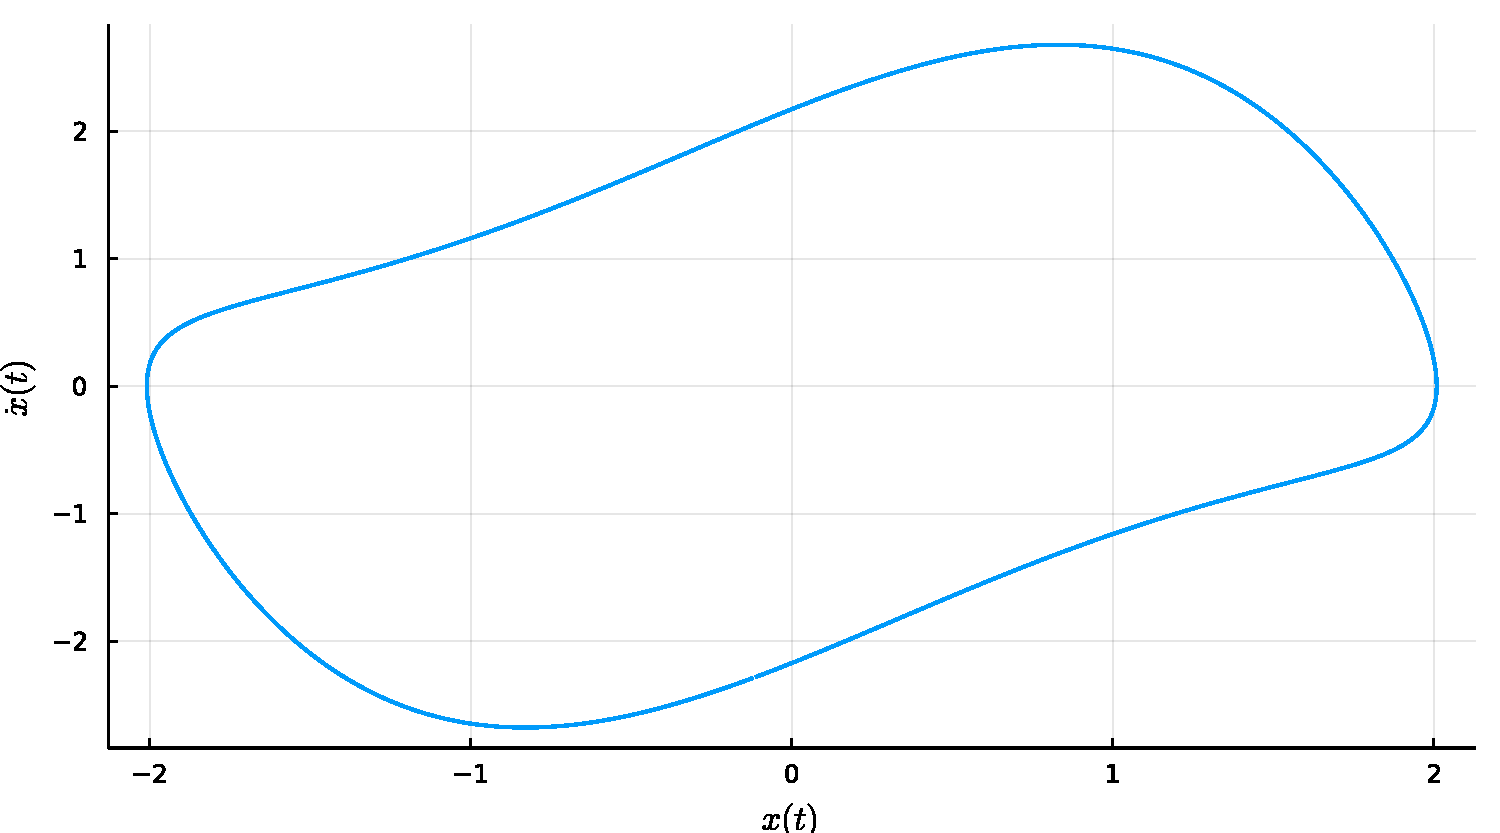
\includegraphics[keepaspectratio,scale = 0.35]{05_ODE/Phase_plot.pdf}
	\caption{Newton法で求めた周期解の位相図\newline \qquad (横軸:$x(t)$, 縦軸:$\dot{x}(t)$)}
	\label{fig:Phase_plot}
	\end{center}
\end{figure}

\begin{figure}[h]
	\centering
	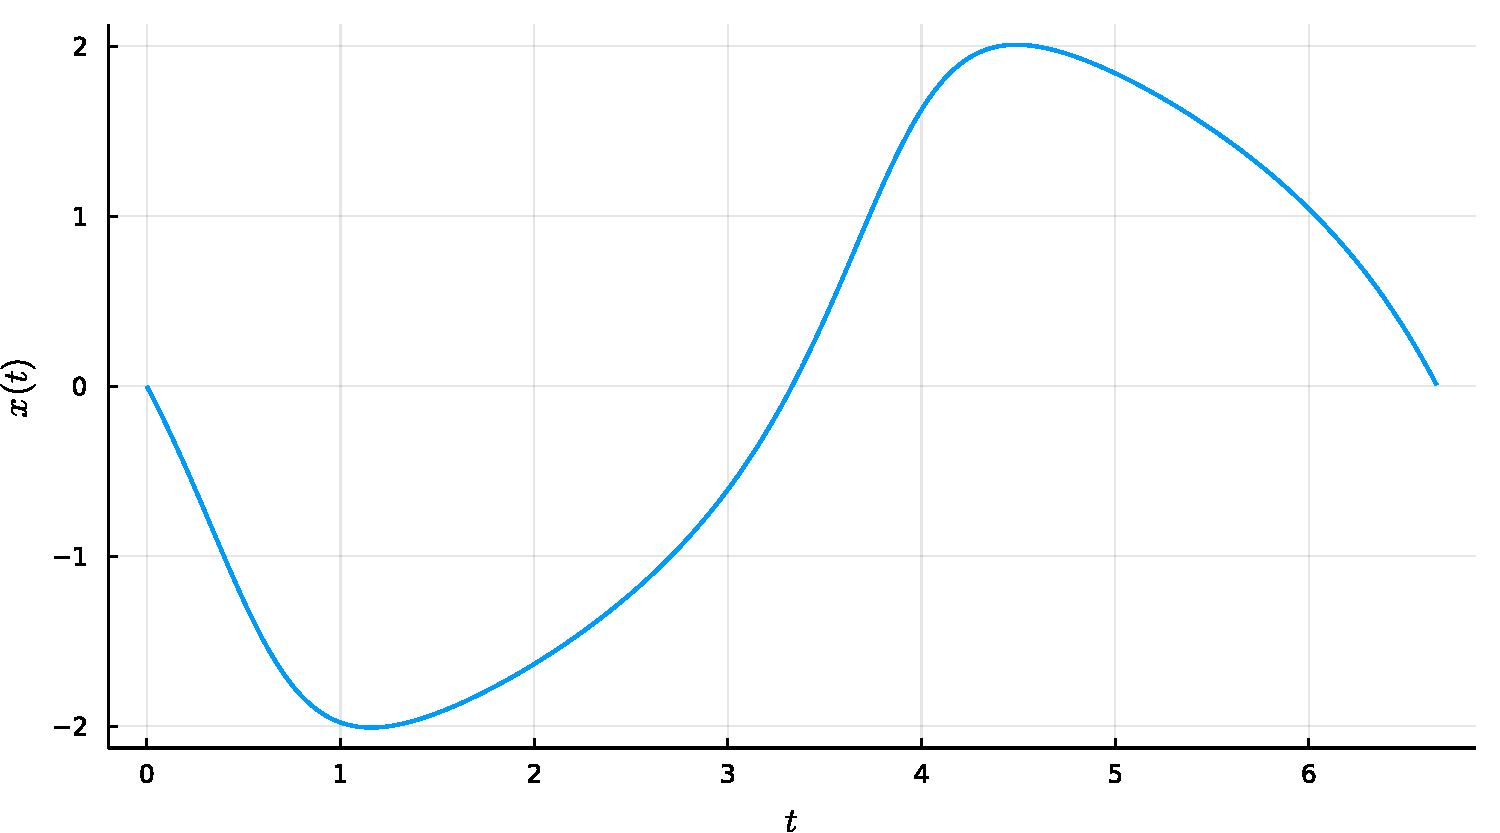
\includegraphics[keepaspectratio,scale = 0.35]{05_ODE/solution.pdf}
	\caption{周期解のプロファイル(横軸:$t$, 縦軸:$x(t)$)}
	\label{fig:solution}
\end{figure}

\begin{figure}[h]
	\centering
	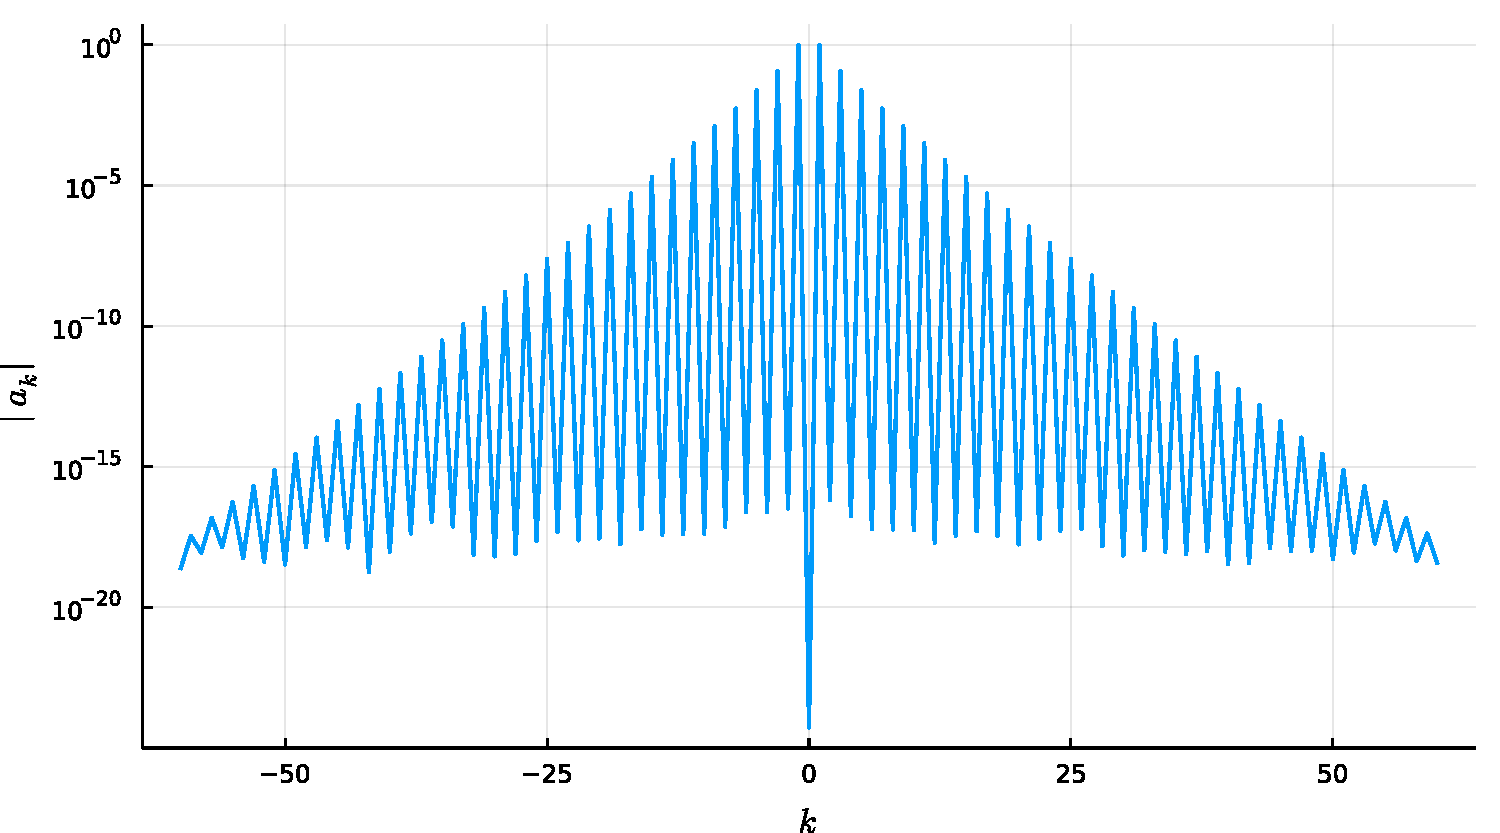
\includegraphics[keepaspectratio,scale = 0.35]{05_ODE/coeffs.pdf}
	\caption{近似周期解のフーリエ係数}
	\label{fig:coeffs}
\end{figure}

\clearpage

フーリエ係数の図を見ると、係数が $10^{-18}$ 程度まで落ちていることがわかり、高精度に近似解を求められていることが期待される。



%\end{document}